%=======================================
% ============== PREAMBLE ============== 
% ======================================

% Beamer Presentation
\documentclass[12pt]{beamer}

% Packages
\usepackage[utf8]{inputenc}
\usepackage[T1]{fontenc}
\usepackage{fontspec}
\usepackage[american]{babel}
\usepackage[autostyle]{csquotes}
\usepackage[natbib=true,backend=biber,isbn=false,maxbibnames=99,doi=false]{biblatex}
\usepackage{graphicx}   % Enable PNG,JPEG import
\usepackage{amsthm}     % Theorems
\usepackage{amsfonts}   % AMS fonts
\usepackage{amsmath}    % AMS math
\usepackage{bm}         % For bold font
\usepackage{alltt}      % Easy verbose environment
\usepackage{fixltx2e}   % Fixes
\usepackage{booktabs}   % Proper tables

% Beamer (LaTeX PDF presentation) stuff
\usetheme{uleiden}
\beamertemplatenavigationsymbolsempty
\setbeamercolor{alerted text}{fg=uleiden}

\frenchspacing  % Only one space after period

\newtheoremstyle{break}% name
  {}%         Space above, empty = `usual value'
  {}%         Space below
  {\normalfont}% Body font
  {}%         Indent amount (empty = no indent, \parindent = para indent)
  {\bfseries}% Thm head font
  {.}%        Punctuation after thm head
  {\newline}% Space after thm head: \newline = linebreak
  {}%         Thm head spec

\theoremstyle{break}
\newtheorem{mydef}{Definition}  % Environment for definitions

% Bibliography and citation
%\addbibresource{/home/benny/Dropbox/seminar/Paper/V3/pagerank_paper.bib}
%\DeclareFieldFormat[inbook,article]{citetitle}{#1}
%\DeclareFieldFormat[inbook,article]{title}{#1}

% Title page
\title{Entity Resolution in Unstructured Data}
\subtitle{and applications in the analysis of historical documents}
\author{Benjamin van der Burgh}
\date{March 15th 2016}


%%% Separation between items in list
\usepackage{etoolbox}% http://ctan.org/pkg/etoolbox

\makeatletter
\patchcmd{\@listI}{\itemsep3\p@}{\itemsep.7em}{}{}
\makeatother


\makeatletter
\newenvironment{customlist}[2]{
  \ifnum\@itemdepth >2\relax\@toodeep\else
      \advance\@itemdepth\@ne%
      \beamer@computepref\@itemdepth%
      \usebeamerfont{itemize/enumerate \beameritemnestingprefix body}%
      \usebeamercolor[fg]{itemize/enumerate \beameritemnestingprefix body}%
      \usebeamertemplate{itemize/enumerate \beameritemnestingprefix body begin}%
      \begin{list}
        {
            \usebeamertemplate{itemize \beameritemnestingprefix item}
        }
        { \leftmargin=#1 \itemindent=#2
            \def\makelabel##1{%
              {%  
                  \hss\llap{{%
                    \usebeamerfont*{itemize \beameritemnestingprefix item}%
                        \usebeamercolor[fg]{itemize \beameritemnestingprefix item}##1}}%
              }%  
            }%  
        }
  \fi
}
{
  \end{list}
  \usebeamertemplate{itemize/enumerate \beameritemnestingprefix body end}%
}
\makeatother



%%% Packages used for nice quoting
\usepackage{etoolbox}
%\usepackage[svgnames]{xcolor}
\usepackage{tikz}
%\usepackage{framed}
\usepackage{libertine} % or any other font package
\newcommand*\quotefont{\fontfamily{LinuxLibertineT-LF}}

%%% Commands used in nice quoting
\newcommand*\quotesize{40}

\newcommand*{\openquote}
   {\tikz[remember picture,overlay,xshift=-4ex,yshift=-2.5ex]
   \node (OQ) {\quotefont\fontsize{\quotesize}{\quotesize}\selectfont``};\kern0pt}

\newcommand*{\closequote}[1]
  {\tikz[remember picture,overlay,xshift=4ex,yshift={#1}]
   \node (CQ) {\quotefont\fontsize{\quotesize}{\quotesize}\selectfont''};}

% select a colour for the shading
\colorlet{shadecolor}{red}

\newcommand*\shadedauthorformat{\emph}

\newcommand*\authoralign[1]{%
  \if#1l
    \def\authorfill{}\def\quotefill{\hfill}
  \else
    \if#1r
      \def\authorfill{\hfill}\def\quotefill{}
    \else
      \if#1c
        \gdef\authorfill{\hfill}\def\quotefill{\hfill}
      \else\typeout{Invalid option}
      \fi
    \fi
  \fi}

\newenvironment{shadequote}[2][l]%
{\authoralign{#1}
\ifblank{#2}
   {\def\shadequoteauthor{}\def\yshift{-2ex}\def\quotefill{\hfill}}
   {\def\shadequoteauthor{\par\authorfill\shadedauthorformat{#2}}\def\yshift{2ex}}
\begin{quote}\openquote}
{\shadequoteauthor\quotefill\closequote{\yshift}\end{quote}}

%\newcommand\mathmacro[1][A]{\ensuremath{{#1}_1}}
\newcommand*{\parsevar}[1]{\ensuremath{\left\{\textrm{#1}\right\}}}

%=======================================
%============ PRESENTATION =============
%=======================================

\begin{document}

\begin{frame}[plain]
\maketitle

\begin{center}
	\footnotesize
	\begin{tabular}[t]{l l}
	Supervisors: & Dr. Arno Knobbe\\
	             & Dr. Siegfried Nijssen
	\end{tabular}%
\end{center}
\end{frame}


%%%%%%% Overview %%%%%%

% Informal introduction to the problem with example (motivation) (2)

\begin{frame}
	\frametitle{Overview}
	
	\begin{enumerate}
		\item Goals of the Traces Through Time project
		\item Format problem description
		\item Record extraction
		\item Comparison of record fields
		\item Candidate pair classification
		\item Maximally k-informative itemsets
		\item Experiments
		\item Conclusions and future work
	\end{enumerate}
\end{frame}


%%%%%%%%%%%%%%%%%%%%%%%%%%%%%%%%%%%%%%%%%%%%%


\begin{frame}
	\frametitle{Traces Through Time (1) -- Context}
	
	\begin{itemize}
		\item The National Archives stores millions of documents.
		\item Many documents have been converted to a digital format. \begin{itemize}
				\item Automatic: Optical Character Recognition (OCR).
				\item Manual: transcribed by hand.
				\end{itemize} 
		\item Connecting pieces of information regarding people is mostly done manually.
		\item Automating this process allows for studying people in all layers of society, not just the aristocracy.
	\end{itemize}
	
\end{frame}


%%%%%%%%%%%%%%%%%%%%%%%%%%%%%%%%%%%%%%%%%%%%%


\begin{frame}

	\begin{shadequote}[r]{Paulo Coelho (The Alchemist)}
		No matter what he does, every person on earth plays a central role in the history of the world. And normally he doesn't know it.
	\end{shadequote}
	
\end{frame}


%%%%%%%%%%%%%%%%%%%%%%%%%%%%%%%%%%%%%%%%%%%%%


\begin{frame}
	\frametitle{Traces Through Time (2) -- Goals}

	\begin{itemize}
		\item Develop a methodology to identify and trace individuals across large and diverse historical datasets.
		\item Look particularly at `fuzzy' data \begin{customlist}{3.5em}{0em}
			\item Aliases: Will, William
			\item Incomplete data: John (only a name)
			\item Spelling variations: Owen, Eoghan
			\item (OCR) Errors: Wihiam (William)
			\end{customlist}
	\end{itemize}
\end{frame}


%%%%%%%%%%%%%%%%%%%%%%%%%%%%%%%%%%%%%%%%%%%%%


\begin{frame}[plain]

	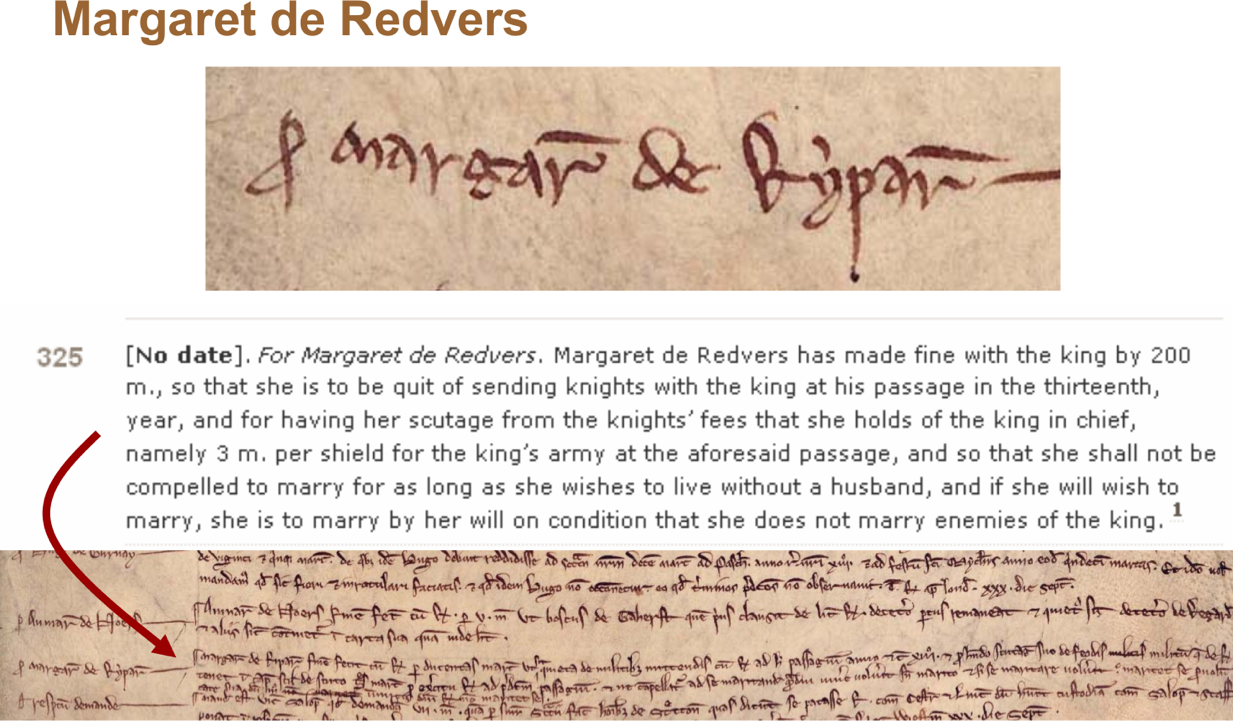
\includegraphics[width=\textwidth]{images/medieval_document}
	
\end{frame}


%%%%%%%%%%%%%%%%%%%%%%%%%%%%%%%%%%%%%%%%%%%%%


\begin{frame}
	\frametitle{Traces Through Time (3) -- Collaboration}
	
	\begin{itemize}
		\item The project set out as a collaboration between several institutes: \begin{itemize}
			\item The National Archives
			\item Institute of Historical Research
			\item Brighton University
			\item Leiden University
			\end{itemize}
		\item Brighton University worked on \emph{Natural Language Processing}.
		\item Our job was to perform record linkage on the extracted references delivered by Brighton University.
	\end{itemize}
	
\end{frame}


%%%%%%%%%%%%%%%%%%%%%%%%%%%%%%%%%%%%%%%%%%%%%

\begin{frame}
	\frametitle{Problem Definition (1)}
	
	\begin{block}{Record}
		A record $r$ is a tuple of $m$ attributes, each having a certain domain, that describes an entity, i.e., $r \in A_1 \times A2 \times \dots \times A_m$.
	\end{block}
	
	\begin{itemize}
	  	\item We assume that records are \alert{descriptions} of people.
	  	\item Records are potentially \alert{ambiguous}: they can describe more than one person.
	\end{itemize}
	
\end{frame}


%%%%%%%%%%%%%%%%%%%%%%%%%%%%%%%%%%%%%%%%%%%%%


\begin{frame}
	\frametitle{Problem Definition (2)}
	
	\begin{block}{Record Linkage}
		Given a set $\mathcal{R}$ of records, determine which of these records refer to the same entity.
	\end{block}
	
	\begin{itemize}
		\item Record linkage is a \alert{binary classification problem}.
		\item Record pairs are classified as \alert{matching} or \alert{non-matching}.
		\item The set of entities is usually unknown.
		\item Even with expert knowledge, it is hard to determine the match status of a record pair.
	\end{itemize}

\end{frame}


%%%%%%%%%%%%%%%%%%%%%%%%%%%%%%%%%%%%%%%%%%%%%


\begin{frame}
	\frametitle{Record Extraction}

	\begin{itemize}
		\item Instead of waiting for input from Brighton University, a simple context-free grammar was written in order to extract occurences.
  		\item First names and articles (of, de la, etc.) were used as anchor points in the text.
  		\item Capitalization, punctuation and ordering define the class of surrounding words.
  	\end{itemize}
  	
  	\begin{center}
  		\parsevar{first name} \parsevar{article} \parsevar{capitalized word} \\
  		$\downarrow$ \\ 
  		\parsevar{first name} \parsevar{article} \parsevar{last name}
  	\end{center}
\end{frame}


%%%%%%%%%%%%%%%%%%%%%%%%%%%%%%%%%%%%%%%%%%%%%


\begin{frame}
	\frametitle{Record Examples}
	
	\begin{quote}
		\footnotesize
		Concerning the corn of \underline{Roger of Hyde}. Order to the \underline{sheriff of Oxfordshire} to make the king’s advantage without delay, by the view of law-worthy men, from all of the corn of \underline{Roger of Hyde, knight}, in Hyde, who is with the Earl Marshal, and to put in gage etc. all those who he will find threshing that corn and intermeddling with the land of the same \underline{Roger} without warrant, to be before the king at his command to answer for it.
	\end{quote}
	
	\begin{table}
		\footnotesize
		\centering
		\begin{tabular}{l l l l l}
	\toprule
	\textbf{Title} & \textbf{First name} & \textbf{Article} & \textbf{Last name} & \textbf{Role} \\
	\midrule
	& Roger & of & Hyde        & \\
	sherrif &       & of & Oxfordshire & \\
	& Roger & of & Hyde        & knight \\
	& Roger &    &             & \\
	\bottomrule
\end{tabular}
		%\caption{A possible segmentation of the paragraph taken from \emph{Fine Roll C 60/33}.}
		%\label{tab:segmentation}
	\end{table}
	
\end{frame}


%%%%%%%%%%%%%%%%%%%%%%%%%%%%%%%%%%%%%%%%%%%%%





% Brief introduction to the goals of the TTT project (goals) (1)
% Formal problem introduction (3)
% Describe the pipeline (note that we strive for a tabular approach?)
%     Record extraction is done by means of a CFG
%     Briefly mention blocking as means of reducing the number of comparisons (show graph that shows benefits).
%     Field-based comparisons: describe some simple means of comparison: Edit distance.
           % ---- Briefly explain advantages and disadvantages of methods without diving into the details.
%     Candidate pair classification (3)

% Feature extraction
%    Give the example of Mr. Carkesse

% Experimental evaluation

% Conclusions and future work



% End slide with picture of thesis front page and URL to GitHub.

% Extra:
% Describe some of the benefits of studying the LaTeX source.
%     Data to be consumed by LaTeX in separate file (model-view approach)
%     Source syntax highlighting and formatting with minted.
%     Proper table formatting with booktabs
%     Doing all graphics with vectorized data formats to ensure a high-quality result.

\end{document}